\providecommand{\qcOne}{\mathbf{1}}   %
\providecommand{\qcor}[1]{\ulcorner#1\urcorner}   %
\providecommand{\ShapeSpan}{\sqcap}    %
\providecommand{\ShapeCospan}{\sqcup}  %
\providecommand{\ShapeSquare}{\square} %

\section{\trLimit{}与\trColimit{}的\trUniversalProperty}\label{sec:universal-property-of-limits-and-colimits}

为了刻画\trLimit{}与\trColimit{}的\trUniversalProperty{}，我们回到定义 2.3.1 的
一般语境，同时考虑取值于某个\trInfinityCategory{}、且由一个\trSimplicialSet{}%
或另一个\trInfinityCategory{}索引的\trDiagram{}，此时要求环境\trInfinityCosmos{}%
\trCartesianClosed{}。正如命题 4.1.1 的情形，定理 3.5.8 立即特化到定义 2.3.8 的
框架，证得：

\begin{proposition}[余/极限表示锥]\label{prop:colimits-represent-cones}
一族\trDiagram{} $d\colon D\to A^{J}$ 容许一个\trLimit{}，当且仅当 $d$ 之上的%
\trInfinityCategoryOfCones{} $\mathrm{Hom}_{A^{J}}(\Delta,d)$ 是右\trRepresentable
\begin{equation*}
\mathrm{Hom}_{A^{J}}(\Delta,d)\simeq_{D\times A}\mathrm{Hom}_{A}(A,\ell),
\end{equation*}
此时表示函子 $\ell\colon D\to A$ 定义出\trLimit{}函子。对偶地，一族\trDiagram{}
$d\colon D\to A^{J}$ 容许一个\trColimit{}，当且仅当 $d$ 之下的%
\trInfinityCategoryOfCones{} $\mathrm{Hom}_{A^{J}}(d,\Delta)$ 是左\trRepresentable
\begin{equation*}
\mathrm{Hom}_{A^{J}}(d,\Delta)\simeq_{A\times D}\mathrm{Hom}_{A}(c,A),
\end{equation*}
此时表示函子 $c\colon D\to A$ 定义出\trColimit{}函子。
\end{proposition}

推论 3.6.10 特化后告诉我们：这样的表示可以由\trTerminal{}\trElement{}或%
\trInitial{}\trElement{}来编码；这一结果在单个\trDiagram{}（而非\trDiagram{}族）
的情形最易解读。

\begin{proposition}[\trLimit{}作为\trTerminal\trCone]\label{prop:limits-as-terminal-cones}
\trInfinityCategory{} $A$ 中形状为 $J$ 的一个\trDiagram{} $d\colon\qcOne\to A^{J}$
(i) 容许一个\trLimit{}，当且仅当 $d$ 之上的\trInfinityCategoryOfCones{}
$\mathrm{Hom}_{A^{J}}(\Delta,d)$ 容许一个\trTerminal{}\trElement{}，此时该%
\trTerminal{}\trElement{}定义一个\trLimit\trCone{}；而
(ii) 容许一个\trColimit{}，当且仅当 $d$ 之下的\trInfinityCategoryOfCones{}
$\mathrm{Hom}_{A^{J}}(d,\Delta)$ 容许一个\trInitial{}\trElement{}，此时该%
\trInitial{}\trElement{}定义\trColimit\trCone{}。
\end{proposition}

\trLimit\trCone{}与\trColimit\trCone{}在同构意义下的唯一性，可由应用引理 2.2.3
得到；亦可从绝对提升图刻画出发证明（见练习 2.3.vi）。

\begin{remark}\label{rem:family-limit-terminal-element}
推论 3.6.10 同样适用于断言：一族\trDiagram{} $d\colon D\to A^{J}$ 容许一个%
\trLimit{}，恰好当 $\mathrm{Hom}_{A^{J}}(\Delta,d)$ 容许一个 $D$ 之上的%
\trTerminal{}\trElement{}；而容许一个\trColimit{}，恰好当
$\mathrm{Hom}_{A^{J}}(d,\Delta)$ 容许一个 $D$ 之上的\trInitial{}\trElement{}。
\end{remark}

出于审美上的理由，下面两个结果我们只对由\trSimplicialSet{}索引的\trDiagram{}%
来陈述，以便使用更优雅、或许更易于解读的记号。正如\cref{ex:j-indexed-versions}
所揭示的，并没有数学上的理由要限制在这一特殊情形。%
\footnote{事实上，证明实际使用的是余定义域投影函子
$p_{1}\colon\mathrm{Hom}_{A^{J}}(\Delta,A^{J})\twoheadrightarrow A^{J}$，而非与之%
\trEquivalence{}的等价纤维化
$\mathrm{res}\colon A^{J^{\triangleleft}}\twoheadrightarrow A^{J}$，因此这一更
朴素的论证同样适用于由\trInfinityCategory{} $J$ 索引\trDiagram{}的情形——无论
其所处的\trCartesianClosed{}\trInfinityCosmos{}是否容许可用于索引形状的联接运算。}

\begin{proposition}\label{prop:absolute-right-lifting-res}
一个\trInfinityCategory{} $A$ 容许由\trSimplicialSet{} $J$ 索引的一族\trDiagram{}
$d\colon D\to A^{J}$ 的\trLimit{}，当且仅当 $d$ 沿限制函子
\begin{center}
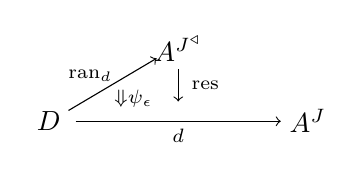
\begin{tikzpicture}[x=1.3em,y=1.3em]
  \node (Ajt) at (3.6,2.0) {$A^{J^{\triangleleft}}$};
  \node (D) at (0,0) {$D$};
  \node (Aj) at (7.2,0) {$A^{J}$};
  \draw[->] (0.55,0.3) -- (3.0,1.75);
  \node at (1.15,1.25) {$\scriptstyle\mathrm{ran}_{d}$};
  \draw[->] (3.6,1.45) -- (3.6,0.55);
  \node at (4.35,1.0) {$\scriptstyle\mathrm{res}$};
  \draw[->] (0.75,0) -- (6.45,0);
  \node at (3.6,-0.4) {$\scriptstyle d$};
  \node at (2.35,0.62) {$\scriptstyle\Downarrow\psi_{\epsilon}$};
\end{tikzpicture}
\end{center}
存在一个绝对右\trLifting{}。当这些等价条件成立时，$\epsilon$ 必为同构，且可取为
恒同。
\end{proposition}

\begin{proof}
依定义 2.3.8，一族\trDiagram{} $d$ 容许一个\trLimit{}，当且仅当它沿
$\Delta\colon A\to A^{J}$ 容许一个绝对右\trLifting{}。依命题 3.6.14，这一绝对提升
存在，当且仅当 $d$ 沿余定义域投影函子
$p_{1}\colon\mathrm{Hom}_{A^{J}}(\Delta,A^{J})\to A^{J}$ 容许一个绝对右\trLifting{}，
此时后一绝对右提升图表的自然同构是可逆的。依推论 4.2.8，限制函子
$\mathrm{res}\colon A^{J^{\triangleleft}}\twoheadrightarrow A^{J}$ \trEquivalence{}于这一余定义域
投影函子，故练习 3.5.ii 蕴含：$d$ 沿 $p_{1}$ 的绝对右提升等价于 $d$ 沿
$\mathrm{res}$ 的绝对右提升。若这一绝对提升图由一个可逆 2-胞腔充实，则命题 1.4.9
所证的等价纤维化的同构提升性质，可用来把函子
$\mathrm{ran}_{d}\colon D\to A^{J^{\triangleleft}}$ 替换为同构的函子，得到一个
严格交换的三角，且依练习 2.3.vi 它仍是绝对右提升图表。
\end{proof}

\cref{prop:absolute-right-lifting-res}特化后给出一个结构化的刻画，针对那些容许
特定形状的一切\trLimit{}或一切\trColimit{}的\trInfinityCategory{}（见定义 2.3.2）。

\begin{corollary}\label{cor:res-fibered-adjoints}
一个\trInfinityCategory{} $A$ 容许由\trSimplicialSet{} $J$ 索引的一切\trLimit{}，
当且仅当左下图的限制函子在 $A^{J}$ 之上容许一个\trFibered\trRightAdjoint{}；而 $A$
容许由\trSimplicialSet{} $J$ 索引的一切\trColimit{}，当且仅当右下图的限制函子在
$A^{J}$ 之上容许一个\trFibered\trLeftAdjoint{}。
\begin{center}
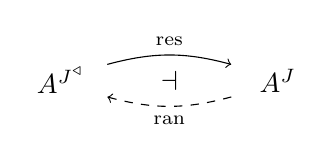
\begin{tikzpicture}[x=1.4em,y=1.4em]
  \node (l) at (0,0) {$A^{J^{\triangleleft}}$};
  \node (r) at (5.6,0) {$A^{J}$};
  \draw[->] (1.2,0.42) to[bend left=15] node[above]{$\scriptstyle\mathrm{res}$} (4.4,0.42);
  \node at (2.8,0) {$\dashv$};
  \draw[->,dashed] (4.4,-0.42) to[bend left=15] node[below]{$\scriptstyle\mathrm{ran}$} (1.2,-0.42);
\end{tikzpicture}
\qquad
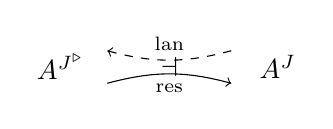
\begin{tikzpicture}[x=1.4em,y=1.4em]
  \node (l) at (0,0) {$A^{J^{\triangleright}}$};
  \node (r) at (5.6,0) {$A^{J}$};
  \draw[->,dashed] (4.4,0.42) to[bend left=15] node[above]{$\scriptstyle\mathrm{lan}$} (1.2,0.42);
  \node at (2.8,0) {$\dashv$};
  \draw[->] (1.2,-0.42) to[bend left=15] node[below]{$\scriptstyle\mathrm{res}$} (4.4,-0.42);
\end{tikzpicture}
\end{center}
\end{corollary}

\begin{proof}
依\cref{prop:absolute-right-lifting-res}与引理 2.3.7，$A$ 容许一切 $J$ 形状的%
\trLimit{}，当且仅当函子 $\mathrm{res}\colon A^{J^{\triangleleft}}\twoheadrightarrow A^{J}$ 容许
一个\trRightAdjoint\trRightInverse{}。由于限制函子是一个等价纤维化，引理 3.6.9
适用，可将该\trRightAdjoint\trRightInverse\trRectify{}为一个\trFibered\trAdjunction{}。
\end{proof}

现在，我们把已发展的一般理论应用到一些特定的索引形状上。

\begin{definition}[\trTensor{}与\trCotensor]\label{def:tensors-cotensors}
设 $K$ 为一个\trSimplicialSet{}，并设 $a\colon\qcOne\to A$ 为某个\trInfinityCategory{}
$A$ 的一个\trElement{}。$a$ 经 $K$ 的\textbf{\trTensor}（tensor）$K\otimes a$，是取值为
$a$ 的常值 $K$-索引\trDiagram{}的\trColimit{}；而 $a$ 经 $K$ 的%
\textbf{\trCotensor}（cotensor）$a^{K}$，则是同一\trDiagram{}的\trLimit{}。于是，
\trTensor{}函子与\trCotensor{}函子可由下列绝对提升图定义：
\begin{center}
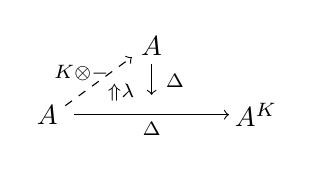
\begin{tikzpicture}[x=1.3em,y=1.3em]
  \node (At) at (2.9,1.9) {$A$};
  \node (Al) at (0,0) {$A$};
  \node (Ak) at (5.8,0) {$A^{K}$};
  \draw[->,dashed] (0.5,0.25) -- (2.35,1.6);
  \node at (0.95,1.15) {$\scriptstyle K\otimes-$};
  \draw[->] (2.9,1.4) -- (2.9,0.55);
  \node at (3.55,0.95) {$\scriptstyle\Delta$};
  \draw[->] (0.75,0) -- (5.05,0);
  \node at (2.9,-0.4) {$\scriptstyle\Delta$};
  \node at (2.05,0.62) {$\scriptstyle\Uparrow\lambda$};
\end{tikzpicture}
\qquad
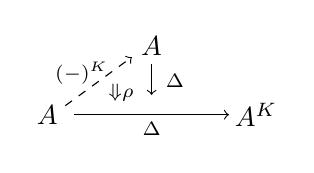
\begin{tikzpicture}[x=1.3em,y=1.3em]
  \node (At) at (2.9,1.9) {$A$};
  \node (Al) at (0,0) {$A$};
  \node (Ak) at (5.8,0) {$A^{K}$};
  \draw[->,dashed] (0.5,0.25) -- (2.35,1.6);
  \node at (0.95,1.15) {$\scriptstyle(-)^{K}$};
  \draw[->] (2.9,1.4) -- (2.9,0.55);
  \node at (3.55,0.95) {$\scriptstyle\Delta$};
  \draw[->] (0.75,0) -- (5.05,0);
  \node at (2.9,-0.4) {$\scriptstyle\Delta$};
  \node at (2.05,0.62) {$\scriptstyle\Downarrow\rho$};
\end{tikzpicture}
\end{center}
依定理 3.5.3，这些绝对提升图定义出纤维化等价
\begin{equation*}
\mathrm{Hom}_{A}(K\otimes-,A)\simeq_{A\times A}\mathrm{Hom}_{A^{K}}(\Delta,\Delta)
\simeq_{A\times A}\mathrm{Hom}_{A}(A,(-)^{K}),
\end{equation*}
二者复合，便定义出编码\trTensor{}函子与\trCotensor{}函子之间一个\trAdjunction{}的%
\trFiberedEquivalence{}：
\begin{center}
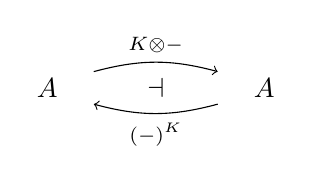
\begin{tikzpicture}[x=1.4em,y=1.4em]
  \node (l) at (0,0) {$A$};
  \node (r) at (5.6,0) {$A$};
  \draw[->] (1.2,0.42) to[bend left=15] node[above]{$\scriptstyle K\otimes-$} (4.4,0.42);
  \node at (2.8,0) {$\dashv$};
  \draw[->] (4.4,-0.42) to[bend left=15] node[below]{$\scriptstyle(-)^{K}$} (1.2,-0.42);
\end{tikzpicture}
\end{center}
依推论 4.1.3，表达\trTensor{}与\trCotensor{}之\trUniversalProperty{}的那些%
\trFiberedEquivalence{}沿元素 $a,x\colon\qcOne\to A$ 作\trPullback{}，定义出%
\trMappingSpace{}的等价：
\begin{equation*}
\begin{gathered}
\mathrm{Hom}_{A}(K\otimes a,x)\cong\mathrm{Hom}_{A^{K}}(\Delta a,\Delta x)
\cong\mathrm{Hom}_{A}(a,x)^{K}\qquad\text{与}\\
\mathrm{Hom}_{A}(x,a^{K})\cong\mathrm{Hom}_{A^{K}}(\Delta x,\Delta a)
\cong\mathrm{Hom}_{A}(x,a)^{K}.
\end{gathered}
\end{equation*}
\end{definition}

\begin{definition}[\trSpan{}与\trCospan]\label{def:span-cospan}
\trInfinityCategory{} $A$ 中的一个\textbf{\trSpan}（span），是由单纯集
$\ShapeSpan:=\Lambda^{0}[2]$ 索引的\trDiagram{}，后者由两条 $1$-单纯形沿其定义域
顶点粘合而成。对偶地，$A$ 中的一个\textbf{\trCospan}（cospan），是由单纯集
$\ShapeCospan:=\Lambda^{2}[2]$ 索引的\trDiagram{}，后者由两条 $1$-单纯形沿其余
定义域顶点粘合而成。\trInfinityCategory{} $A$ 中的余跨度与跨度，可分别由把一对
箭头沿其公共余定义域或公共定义域粘合而定义：

\begin{center}
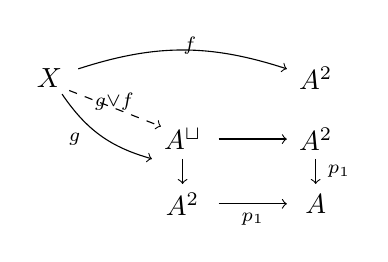
\begin{tikzpicture}[x=1.3em,y=1.3em]
  \node (X) at (0,2.6) {$X$};
  \node (Art) at (7.4,2.6) {$A^{2}$};
  \node (Acup) at (3.7,0.9) {$A^{\ShapeCospan}$};
  \node (Arm) at (7.4,0.9) {$A^{2}$};
  \node (Ab) at (3.7,-0.9) {$A^{2}$};
  \node (A) at (7.4,-0.9) {$A$};
  \draw[->] (0.8,2.85) to[bend left=18] (6.6,2.85);
  \node at (3.9,3.5) {$\scriptstyle f$};
  \draw[->,dashed] (0.55,2.25) -- (3.1,1.25);
  \node at (1.8,1.95) {$\scriptstyle g\vee f$};
  \draw[->] (0.35,2.15) to[bend right=20] (2.85,0.35);
  \node at (0.7,0.9) {$\scriptstyle g$};
  \draw[->] (4.7,0.9) -- (6.6,0.9);
  \draw[->] (3.7,0.35) -- (3.7,-0.35);
  \draw[->] (7.4,0.35) -- (7.4,-0.35);
  \node at (8.05,0.0) {$\scriptstyle p_{1}$};
  \draw[->] (4.7,-0.9) -- (6.6,-0.9);
  \node at (5.65,-1.32) {$\scriptstyle p_{1}$};
  \node at (5.1,0.35) {$\scriptstyle\lrcorner$};
\end{tikzpicture}
\qquad
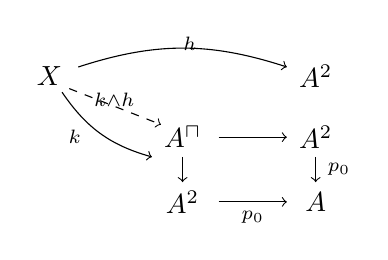
\begin{tikzpicture}[x=1.3em,y=1.3em]
  \node (X) at (0,2.6) {$X$};
  \node (Art) at (7.4,2.6) {$A^{2}$};
  \node (Acup) at (3.7,0.9) {$A^{\ShapeSpan}$};
  \node (Arm) at (7.4,0.9) {$A^{2}$};
  \node (Ab) at (3.7,-0.9) {$A^{2}$};
  \node (A) at (7.4,-0.9) {$A$};
  \draw[->] (0.8,2.85) to[bend left=18] (6.6,2.85);
  \node at (3.9,3.5) {$\scriptstyle h$};
  \draw[->,dashed] (0.55,2.25) -- (3.1,1.25);
  \node at (1.8,1.95) {$\scriptstyle k\wedge h$};
  \draw[->] (0.35,2.15) to[bend right=20] (2.85,0.35);
  \node at (0.7,0.9) {$\scriptstyle k$};
  \draw[->] (4.7,0.9) -- (6.6,0.9);
  \draw[->] (3.7,0.35) -- (3.7,-0.35);
  \draw[->] (7.4,0.35) -- (7.4,-0.35);
  \node at (8.05,0.0) {$\scriptstyle p_{0}$};
  \draw[->] (4.7,-0.9) -- (6.6,-0.9);
  \node at (5.65,-1.32) {$\scriptstyle p_{0}$};
  \node at (5.1,0.35) {$\scriptstyle\lrcorner$};
\end{tikzpicture}
\end{center}
\end{definition}

\begin{definition}[\trPushout{}与\trPullback]\label{def:pushout-pullback}
\trInfinityCategory{} $A$ 中的一个\textbf{\trPushout}（pushout），是由单纯集
$\ShapeSpan$ 索引的\trDiagram{}的\trColimit{}；而一个\textbf{\trPullback}
（pullback）则是\trInfinityCategory{} $A$ 中由单纯集 $\ShapeCospan$ 索引的%
\trDiagram{}的\trLimit{}。形状为 $\ShapeCospan$ 的\trDiagram{}之上的\trCone{}或
形状为 $\ShapeSpan$ 的\trDiagram{}之下的\trCone{}，定义出\textbf{交换方块}
（commutative squares），即形状为
\begin{equation*}
\ShapeSquare:=\ShapeSpan^{\triangleright}\cong 2\times 2\cong\ShapeCospan^{\triangleleft}
\end{equation*}
的\trDiagram{}。

\trInfinityCategory{} $A$ 中的一个\textbf{拉回方块}（pullback square），是
$A^{\ShapeSquare}$ 的一个\trElement{}，它定义出其底下的余跨度的一个绝对右\trLifting{}：
\begin{center}
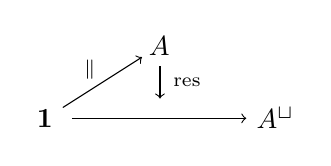
\begin{tikzpicture}[x=1.3em,y=1.3em]
  \node (Asq) at (3.2,2.0) {$A^{\ShapeSquare}$};
  \node (One) at (0,0) {$\qcOne$};
  \node (Acup) at (6.4,0) {$A^{\ShapeCospan}$};
  \draw[->] (0.5,0.3) -- (2.7,1.7);
  \node at (1.25,1.35) {$\scriptstyle\parallel$};
  \draw[->] (3.2,1.45) -- (3.2,0.55);
  \node at (3.95,1.0) {$\scriptstyle\mathrm{res}$};
  \draw[->] (0.75,0) -- (5.6,0);
\end{tikzpicture}
\qquad
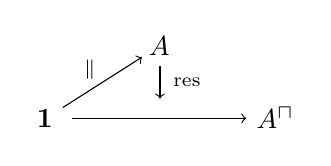
\begin{tikzpicture}[x=1.3em,y=1.3em]
  \node (Asq) at (3.2,2.0) {$A^{\ShapeSquare}$};
  \node (One) at (0,0) {$\qcOne$};
  \node (Acup) at (6.4,0) {$A^{\ShapeSpan}$};
  \draw[->] (0.5,0.3) -- (2.7,1.7);
  \node at (1.25,1.35) {$\scriptstyle\parallel$};
  \draw[->] (3.2,1.45) -- (3.2,0.55);
  \node at (3.95,1.0) {$\scriptstyle\mathrm{res}$};
  \draw[->] (0.75,0) -- (5.6,0);
\end{tikzpicture}
\end{center}
当 $A$ 容许一切\trPullback{}时，拉回方块可以刻画为 $A^{\ShapeSquare}$ 中使%
\cref{cor:res-fibered-adjoints}的\trAdjunction{} $\mathrm{res}\dashv\mathrm{ran}$
之\trUnit{}分量为同构的那些\trElement{}（见\cref{ex:family-pullback-criteria}）。
对偶地，$A$ 中的一个\textbf{推出方块}（pushout square），是 $A^{\ShapeSquare}$ 的
一个\trElement{}，它定义出其底下的跨度的一个绝对左\trLifting{}，亦即使\trAdjunction
$\mathrm{lan}\dashv\mathrm{res}$ 之\trCounit{}分量为同构的\trElement{}。由推出方块
或拉回方块构成的一族 $X\to A^{\ShapeSquare}$ 之概念可类似定义。
\end{definition}

拉回方块可用绝对提升图来刻画，这对建立它们的基本演算颇为有用。为此，我们使用
下述引理。

\begin{lemma}\label{lem:postcomposition}
考虑一族箭头 $f\colon X\to A^{2}$，它表示一个自然变换
\begin{center}
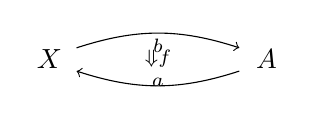
\begin{tikzpicture}[x=1.4em,y=1.2em]
  \node (X) at (0,0) {$X$};
  \node (A) at (5.6,0) {$A$};
  \draw[->] (0.7,0.35) to[bend left=18] (4.9,0.35);
  \node at (2.8,0.42) {$\scriptstyle b$};
  \node at (2.8,0.02) {$\scriptstyle\Downarrow f$};
  \draw[->] (4.9,-0.35) to[bend left=18] (0.7,-0.35);
  \node at (2.8,-0.68) {$\scriptstyle a$};
\end{tikzpicture}
\end{center}
那么存在一个跨度
\begin{center}
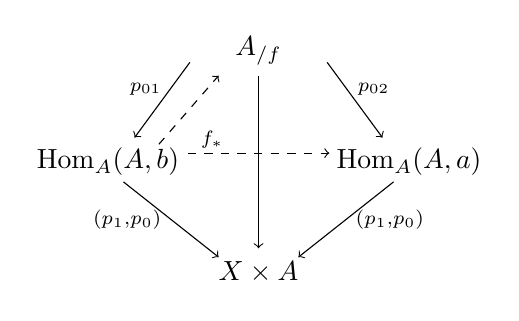
\begin{tikzpicture}[x=1.6em,y=1.6em]
  \node (Af) at (3.4,2.5) {$A_{/f}$};
  \node (Hb) at (0,0) {$\mathrm{Hom}_{A}(A,b)$};
  \node (Ha) at (6.8,0) {$\mathrm{Hom}_{A}(A,a)$};
  \node (XA) at (3.4,-2.5) {$X\times A$};
  \draw[->] (1.85,2.25) -- (0.6,0.55);
  \node at (0.85,1.65) {$\scriptstyle p_{01}$};
  \draw[->] (4.95,2.25) -- (6.2,0.55);
  \node at (6.0,1.65) {$\scriptstyle p_{02}$};
  \draw[->,dashed] (1.15,0.4) -- (2.5,1.95);%
  \draw[->,dashed] (1.8,0.2) -- (5.0,0.2);
  \node at (2.35,0.5) {$\scriptstyle f_{*}$};
  \draw[->] (3.4,1.95) -- (3.4,-1.95);
  \draw[->] (0.35,-0.45) -- node[left]{$\scriptstyle(p_{1},p_{0})$} (2.5,-2.15);
  \draw[->] (6.45,-0.45) -- node[right]{$\scriptstyle(p_{1},p_{0})$} (4.3,-2.15);
\end{tikzpicture}
\end{center}
使得任何到平凡纤维化 $p_{01}$ 的截面与 $p_{02}$ 复合，都定义出一个表示以 $f$ 作%
\trPostComposition{}的函子 $f_{*}$；而且 $f_{*}$ 的\trFiberedIsomorphism{}类中的
每个函子都按此方式产生。%
\footnote{推论 3.5.11 在\trHomotopyTwoCategory{}中的自然变换
$\alpha\colon b\Rightarrow a$ 与函子
$\qcor{\alpha_{*}}\colon\mathrm{Hom}_{A}(A,b)\to\mathrm{Hom}_{A}(A,a)$ 之间，在%
\trFiberedIsomorphism{}的意义下定义了一个双射。此处我们稍稍改变记号，因为我们是
从一族箭头 $f\colon X\to A^{2}$ 出发，而非从该族所表示的那个自然变换出发。}
此外，$f$ 表示一个自然同构 $f\colon b\cong a$，\footnote{原书印作
『$f:a\cong b$』，与其所示自然变换 $f\colon b\Rightarrow a$ 方向相悖，疑为笔误，
此处径改。——译者注}当且仅当等价纤维化 $p_{02}$ 是一个平凡纤维化。
\end{lemma}

\begin{proof}
通过构造每一列的拉回，下方的余跨度之跨度便定义出陈述中那个跨度的对象与映射：
\begin{center}
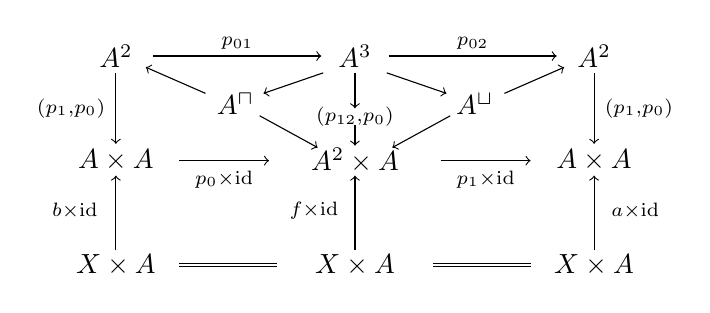
\begin{tikzpicture}[x=1.35em,y=1.35em]
  \node (A2l) at (-6.4,3.2) {$A^{2}$};
  \node (A3) at (0,3.2) {$A^{3}$};
  \node (A2r) at (6.4,3.2) {$A^{2}$};
  \node (Asp) at (-3.2,1.9) {$A^{\ShapeSpan}$};
  \node (Acsp) at (3.2,1.9) {$A^{\ShapeCospan}$};
  \node (AAl) at (-6.4,0.4) {$A\times A$};
  \node (AAm) at (0,0.4) {$A^{2}\times A$};
  \node (AAr) at (6.4,0.4) {$A\times A$};
  \node (XAl) at (-6.4,-2.4) {$X\times A$};
  \node (XAm) at (0,-2.4) {$X\times A$};
  \node (XAr) at (6.4,-2.4) {$X\times A$};
  \draw[->] (-5.4,3.2) -- (-0.9,3.2);
  \node at (-3.15,3.55) {$\scriptstyle p_{01}$};
  \draw[->] (0.9,3.2) -- (5.4,3.2);
  \node at (3.15,3.55) {$\scriptstyle p_{02}$};
  \draw[->] (-0.85,2.75) -- (-2.45,2.2);
  \draw[->] (0.85,2.75) -- (2.45,2.2);
  \draw[->] (-4.0,2.2) -- (-5.6,2.9);
  \draw[->] (4.0,2.2) -- (5.6,2.9);
  \draw[->] (-2.55,1.6) -- (-1.0,0.75);
  \draw[->] (2.55,1.6) -- (1.0,0.75);
  \draw[->] (0,2.75) -- (0,1.8);
  \draw[->] (0,1.35) -- (0,0.8);
  \node at (0,1.58) {$\scriptstyle(p_{12},p_{0})$};
  \node at (-3.9,1.4) {$\scriptstyle\lrcorner$};
  \node at (3.9,1.4) {$\scriptstyle\lrcorner$};
  \draw[->] (-6.4,2.75) -- (-6.4,0.85);
  \node at (-7.6,1.8) {$\scriptstyle(p_{1},p_{0})$};
  \draw[->] (6.4,2.75) -- (6.4,0.85);
  \node at (7.6,1.8) {$\scriptstyle(p_{1},p_{0})$};
  \draw[->] (-4.7,0.4) -- (-2.3,0.4);
  \node at (-3.5,-0.1) {$\scriptstyle p_{0}\times\mathrm{id}$};
  \draw[->] (2.3,0.4) -- (4.7,0.4);
  \node at (3.5,-0.1) {$\scriptstyle p_{1}\times\mathrm{id}$};
  \draw[->] (-6.4,-2.0) -- (-6.4,0.0);
  \node at (-7.5,-0.95) {$\scriptstyle b\times\mathrm{id}$};
  \draw[->] (0,-2.0) -- (0,0.0);
  \node at (-1.1,-0.95) {$\scriptstyle f\times\mathrm{id}$};
  \draw[->] (6.4,-2.0) -- (6.4,0.0);
  \node at (7.5,-0.95) {$\scriptstyle a\times\mathrm{id}$};
  \draw[double] (-4.7,-2.4) -- (-2.1,-2.4);
  \draw[double] (2.1,-2.4) -- (4.7,-2.4);
\end{tikzpicture}
\end{center}
注意，上方两个方块中到诸拉回的映射分别定义出一个平凡纤维化与一个等价纤维化。
于是，依命题 C.1.12，诱导映射
$p_{01}\colon A_{/f}\twoheadrightarrow\mathrm{Hom}_{A}(A,b)$ 是一个平凡纤维化，
而诱导映射 $p_{02}\colon A_{/f}\twoheadrightarrow\mathrm{Hom}_{A}(A,a)$ 是一个
等价纤维化。
特别地，从下方左侧的诸拉回可见：到平凡纤维化 $p_{01}$ 的那些截面，对应于把
可复合箭头对 $\phi\colon\mathrm{Hom}_{A}(A,b)\to A^{2}$ 与
$fp_{1}\colon\mathrm{Hom}_{A}(A,b)\to A^{2}$ 扩充为
$\mathrm{Fun}(\mathrm{Hom}_{A}(A,b),A)$ 中某个 $2$-单纯形的那些映射
$\mathrm{Hom}_{A}(A,b)\to A^{3}$：
\begin{center}
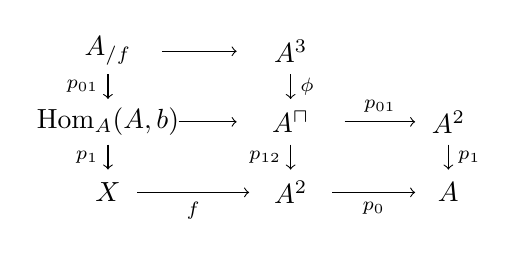
\begin{tikzpicture}[x=1.5em,y=1.5em]
  \node (Af) at (0,3.4) {$A_{/f}$};
  \node (A3t) at (4.4,3.4) {$A^{3}$};
  \node (Hb) at (0,1.7) {$\mathrm{Hom}_{A}(A,b)$};
  \node (Acap) at (4.4,1.7) {$A^{\ShapeSpan}$};
  \node (A2m) at (8.2,1.7) {$A^{2}$};
  \node (X) at (0,0) {$X$};
  \node (A2b) at (4.4,0) {$A^{2}$};
  \node (Ab) at (8.2,0) {$A$};
  \draw[->] (1.3,3.4) -- (3.1,3.4);
  \node at (1.6,2.4) {$\scriptstyle\lrcorner$};
  \draw[->] (0,2.85) -- node[left]{$\scriptstyle p_{01}$} (0,2.25);
  \draw[->] (4.4,2.85) -- node[right]{$\scriptstyle\phi$} (4.4,2.25);
  \draw[->] (1.7,1.7) -- (3.1,1.7);
  \draw[->] (5.7,1.7) -- node[above]{$\scriptstyle p_{01}$} (7.4,1.7);
  \draw[->] (4.4,1.15) -- node[left]{$\scriptstyle p_{12}$} (4.4,0.55);
  \node at (6.2,0.7) {$\scriptstyle\lrcorner$};
  \draw[->] (8.2,1.15) -- node[right]{$\scriptstyle p_{1}$} (8.2,0.55);
  \draw[->] (0,1.15) -- node[left]{$\scriptstyle p_{1}$} (0,0.55);%
  \draw[->] (0.7,0) -- node[below]{$\scriptstyle f$} (3.4,0);
  \draw[->] (5.4,0) -- node[below]{$\scriptstyle p_{0}$} (7.4,0);
\end{tikzpicture}
\qquad
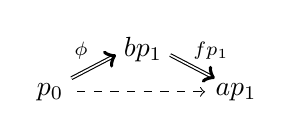
\begin{tikzpicture}[x=1.4em,y=1.4em]
  \node (p0) at (0,0) {$p_{0}$};
  \node (bp1) at (2.4,1.1) {$bp_{1}$};
  \node (ap1) at (4.8,0) {$ap_{1}$};
  \draw[->,double] (0.55,0.35) -- (1.7,0.95);
  \node at (0.8,1.05) {$\scriptstyle\phi$};
  \draw[->,double] (3.1,0.95) -- (4.25,0.35);
  \node at (4.15,1.05) {$\scriptstyle fp_{1}$};
  \draw[->,dashed] (0.7,0) -- (4.0,0);
\end{tikzpicture}
\end{center}
类似地，拉回
\begin{center}
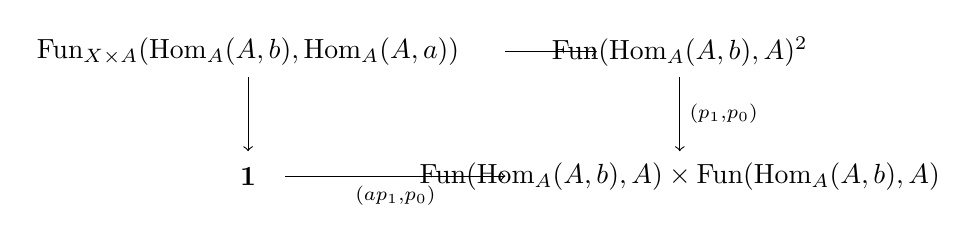
\begin{tikzpicture}[x=1.5em,y=1.5em]
  \node (tl) at (0,1.5) {$\mathrm{Fun}_{X\times A}(\mathrm{Hom}_{A}(A,b),\mathrm{Hom}_{A}(A,a))$};
  \node (tr) at (10.4,1.5) {$\mathrm{Fun}(\mathrm{Hom}_{A}(A,b),A)^{2}$};
  \node (bl) at (0,-1.5) {$\qcOne$};
  \node (br) at (10.4,-1.5) {$\mathrm{Fun}(\mathrm{Hom}_{A}(A,b),A)\times\mathrm{Fun}(\mathrm{Hom}_{A}(A,b),A)$};
  \draw[->] (6.2,1.5) -- (8.4,1.5);
  \draw[->] (0,0.9) -- (0,-0.9);
  \node at (1.4,0) {$\scriptstyle\lrcorner$};
  \draw[->] (10.4,0.9) -- node[right]{$\scriptstyle(p_{1},p_{0})$} (10.4,-0.9);
  \draw[->] (0.9,-1.5) -- node[below]{$\scriptstyle(ap_{1},p_{0})$} (6.2,-1.5);
\end{tikzpicture}
\end{center}
表明：函子 $f_{*}\colon\mathrm{Hom}_{A}(A,b)\to\mathrm{Hom}_{A}(A,a)$ 对应于为
复合箭头选取代表 $fp_{1}\cdot\phi\colon\mathrm{Hom}_{A}(A,b)\to A^{2}$（与推论
3.5.11 的证明比较）。于是，每个截面都在函子的正确\trFiberedIsomorphism{}类中
定义出一个映射；反之，由于 $\mathrm{hFun}(\mathrm{Hom}_{A}(A,b),A)$ 中定义交换
图的每组三元箭头都在 $\mathrm{Fun}(\mathrm{Hom}_{A}(A,b),A)$ 中界定出某个
$2$-单纯形（见引理 1.1.12），每个表示性的函子都按此方式产生。

最后，依练习 3.6.ii 与推论 3.5.11：$f\colon b\Rightarrow a$ 是同构，当且仅当函子
\allowbreak$f_{*}\colon\mathrm{Hom}_{A}(A,b)\to\allowbreak\mathrm{Hom}_{A}(A,a)$
是一个\trFiberedEquivalence{}；而由\trTwoOfThreeProperty{}，$f$ 是同构，当且仅当
$p_{02}$ 是一个平凡纤维化。
\end{proof}

\begin{lemma}[作为绝对提升图的拉回方块]\label{lem:pullbacks-as-absolute-liftings}
\trInfinityCategory{} $A$ 中的一个交换方块是一个拉回方块，当且仅当其诱导的自然变换
$(\mathrm{id}_{a},v)$ 构成一个绝对右提升图表
\begin{center}
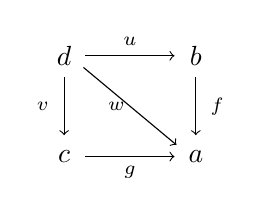
\begin{tikzpicture}[x=1.4em,y=1.4em]
  \node (d) at (0,1.7) {$d$};
  \node (b) at (3.4,1.7) {$b$};
  \node (c) at (0,-0.9) {$c$};
  \node (a) at (3.4,-0.9) {$a$};
  \draw[->] (0.55,1.7) -- (2.85,1.7);
  \node at (1.7,2.08) {$\scriptstyle u$};
  \draw[->] (0,1.15) -- (0,-0.35);
  \node at (-0.55,0.4) {$\scriptstyle v$};
  \draw[->] (3.4,1.15) -- (3.4,-0.35);
  \node at (3.95,0.4) {$\scriptstyle f$};
  \draw[->] (0.55,-0.9) -- (2.85,-0.9);
  \node at (1.7,-1.3) {$\scriptstyle g$};
  \draw[->] (0.5,1.4) -- (2.9,-0.6);
  \node at (1.35,0.4) {$\scriptstyle w$};
\end{tikzpicture}
\qquad
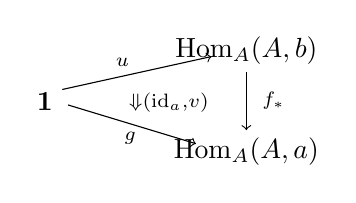
\begin{tikzpicture}[x=1.4em,y=1.4em]
  \node (Hb) at (5.2,1.7) {$\mathrm{Hom}_{A}(A,b)$};
  \node (One) at (0,0.4) {$\qcOne$};
  \node (Ha) at (5.2,-0.9) {$\mathrm{Hom}_{A}(A,a)$};
  \draw[->] (0.45,0.7) -- (4.3,1.55);
  \node at (2.0,1.4) {$\scriptstyle u$};
  \node at (3.2,0.35) {$\scriptstyle\Downarrow(\mathrm{id}_{a},v)$};
  \draw[->] (5.2,1.15) -- (5.2,-0.35);
  \node at (5.9,0.4) {$\scriptstyle f_{*}$};
  \draw[->] (0.6,0.3) -- (3.9,-0.7);
  \node at (2.2,-0.55) {$\scriptstyle g$};
\end{tikzpicture}
\end{center}
\end{lemma}

该陈述需要一些解释。\trInfinityCategory{} $A$ 中的一个交换方块
$s\colon\qcOne\to A^{\ShapeSquare}$ 定义了 $\mathrm{Fun}(\qcOne,A)^{\ShapeSquare}$
的一个元素，其数据由四个顶点 $d$、$b$、$c$、$a\colon\qcOne\to A$ 与五个 $1$-单纯形
$u$、$v$、$f$、$g$、$w\colon\qcOne\to A^{2}$ 给出——它们位于 $A$ 的%
\trUnderlyingQuasiCategory{} $A_{0}:=\mathrm{Fun}(\qcOne,A)$ 之中，如上左图所示
——连同未命名的一对 $2$-单纯形，后者在 $\mathrm{h}A:=\mathrm{hFun}(\qcOne,A)$ 中
见证交换性 $fu=w=gv$。依命题 3.4.7，复合 $f_{*}u$ 同构于 $fu$。依%
\trTwoCellInduction{}，如上右图所示的自然变换 $(\mathrm{id}_{a},v)\colon fu\Rightarrow g$
可通过指明其定义域与余定义域分量来构造，前者我们取为 $v\colon d\Rightarrow c$，
后者我们取为 $\mathrm{id}_{a}$。

\begin{proof}
依推论 4.2.8，限制函子
\begin{center}
\begin{tikzpicture}[x=1.5em,y=1.5em]
  \node (tl) at (0,1.5) {$A^{\ShapeSquare}_{g\vee f}$};
  \node (tr) at (5.4,1.5) {$A^{\ShapeSquare}$};
  \node (bl) at (0,-1.5) {$\qcOne$};
  \node (br) at (5.4,-1.5) {$A^{\ShapeCospan}$};
  \draw[->] (1.75,1.5) -- (3.9,1.5);
  \draw[->] (0,0.9) -- (0,-0.9);
  \node at (1.5,0.1) {$\scriptstyle\lrcorner$};
  \draw[->] (5.4,0.9) -- node[right]{$\scriptstyle\mathrm{res}$} (5.4,-0.9);
  \draw[->] (1.0,-1.5) -- node[below]{$\scriptstyle g\vee f$} (4.5,-1.5);
\end{tikzpicture}
\end{center}
的\trFiber{}等价于余跨度图 $g\vee f$ 之上的\trInfinityCategoryOfCones{}。依%
\cref{prop:limits-as-terminal-cones}，要证明交换方块定义一个拉回图，就是要证明
$(v,f,u,g)\colon\qcOne\to A^{\ShapeSquare}_{g\vee f}$ 定义一个\trTerminal{}\trElement{}。
类似地，依推论 3.6.10，二元组 $(u,(\mathrm{id}_{a},v))$ 定义一个绝对右提升图表，
当且仅当它在逗号∞-范畴 $\mathrm{Hom}_{\mathrm{Hom}_{A}(A,a)}(f_{*},g)$ 中表示一个%
\trTerminal{}\trElement{}。我们宣称：$A^{\ShapeSquare}_{g\vee f}$ 与
$\mathrm{Hom}_{\mathrm{Hom}_{A}(A,a)}(f_{*},g)$ 经由识别这些元素的映射而%
\trEquivalence{}，这就证明了双条件。

为看出这一点，注意单纯方块 $\ShapeSquare$ 可以由沿其对角边粘合两个 $2$-单纯形
而构成，这就给出左下方的拉回：
\begin{center}
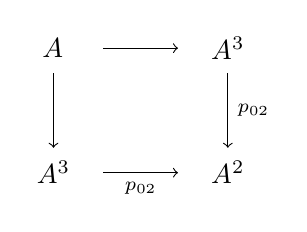
\begin{tikzpicture}[x=1.5em,y=1.5em]
  \node (tl) at (0,1.5) {$A^{\ShapeSquare}$};
  \node (tr) at (4.2,1.5) {$A^{3}$};
  \node (bl) at (0,-1.5) {$A^{3}$};
  \node (br) at (4.2,-1.5) {$A^{2}$};
  \draw[->] (1.2,1.5) -- (3.0,1.5);
  \draw[->] (0,0.9) -- (0,-0.9);
  \node at (1.4,0.1) {$\scriptstyle\lrcorner$};
  \draw[->] (4.2,0.9) -- node[right]{$\scriptstyle p_{02}$} (4.2,-0.9);
  \draw[->] (1.2,-1.5) -- node[below]{$\scriptstyle p_{02}$} (3.0,-1.5);
\end{tikzpicture}
\qquad
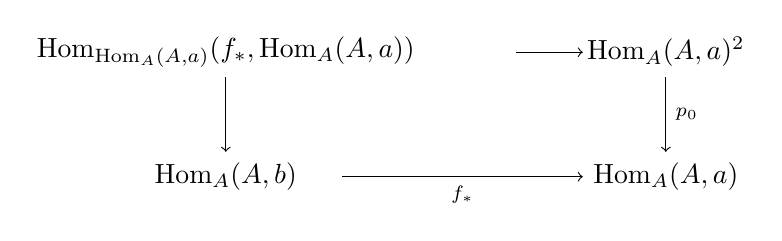
\begin{tikzpicture}[x=1.5em,y=1.5em]
  \node (tl) at (0,1.5) {$\mathrm{Hom}_{\mathrm{Hom}_{A}(A,a)}(f_{*},\mathrm{Hom}_{A}(A,a))$};
  \node (tr) at (10.6,1.5) {$\mathrm{Hom}_{A}(A,a)^{2}$};
  \node (bl) at (0,-1.5) {$\mathrm{Hom}_{A}(A,b)$};
  \node (br) at (10.6,-1.5) {$\mathrm{Hom}_{A}(A,a)$};
  \draw[->] (7.0,1.5) -- (8.6,1.5);
  \draw[->] (0,0.9) -- (0,-0.9);
  \node at (1.7,0.1) {$\scriptstyle\lrcorner$};
  \draw[->] (10.6,0.9) -- node[right]{$\scriptstyle p_{0}$} (10.6,-0.9);
  \draw[->] (2.8,-1.5) -- node[below]{$\scriptstyle f_{*}$} (8.6,-1.5);
\end{tikzpicture}
\end{center}
我们论证：其拉回定义出上方右侧所展示的逗号∞-范畴的那个余跨度中的诸映射，各自
等价于函子 $p_{02}\colon A^{3}\to A^{2}$ 到适当\trFiber{}上的诸拉回。依%
\cref{lem:postcomposition}，映射 $p_{02}\colon A^{3}\to A^{2}$ 在 $f$ 与 $a$ 之上
的诸\trFiber{}上分别拉回到一个等价于 $f_{*}$ 的映射，故只需考虑映射 $p_{0}$。

对定义 $\mathrm{Hom}_{A}(A,a)$ 的拉回图应用 $(-)^{2}$，便得到一个可分解为两个
拉回之复合的拉回方块：
\begin{center}
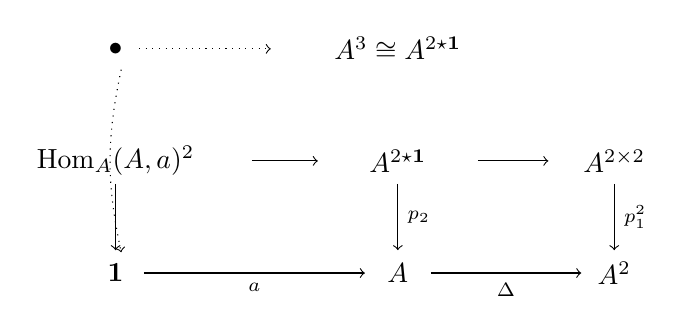
\begin{tikzpicture}[x=1.7em,y=1.5em]
  \node (dot) at (0,2.7) {$\bullet$};
  \node (A3t) at (6.0,2.7) {$A^{3}\cong A^{2\star\qcOne}$};
  \node (Hom2) at (0,0) {$\mathrm{Hom}_{A}(A,a)^{2}$};
  \node (Ast) at (6.0,0) {$A^{2\star\qcOne}$};
  \node (Asq2) at (10.6,0) {$A^{2\times 2}$};
  \node (One) at (0,-2.7) {$\qcOne$};
  \node (A) at (6.0,-2.7) {$A$};
  \node (A2) at (10.6,-2.7) {$A^{2}$};
  \draw[->,dotted] (0.5,2.7) -- (3.3,2.7);
  \draw[->,dotted] (0.12,2.2) to[bend right=12] (0.12,-2.2);
  \draw[->] (2.9,0) -- (4.3,0);
  \draw[->] (7.7,0) -- (9.2,0);
  \draw[->] (0,-0.55) -- (0,-2.15);
  \node at (1.5,-0.75) {$\scriptstyle\lrcorner$};
  \draw[->] (6.0,-0.55) -- node[right]{$\scriptstyle p_{2}$} (6.0,-2.15);
  \node at (8.0,-0.75) {$\scriptstyle\lrcorner$};
  \draw[->] (10.6,-0.55) -- node[right]{$\scriptstyle p_{1}^{2}$} (10.6,-2.15);
  \draw[->] (0.6,-2.7) -- node[below]{$\scriptstyle a$} (5.3,-2.7);
  \draw[->] (6.7,-2.7) -- node[below]{$\scriptstyle\Delta$} (9.9,-2.7);
\end{tikzpicture}
\end{center}
依命题 4.2.7 的等价 $A^{2\star\qcOne}\simeq A^{2\diamond\qcOne}$，左边的拉回方块
表明 $\mathrm{Hom}_{A}(A,a)^{2}$ 等价于 $p_{2}\colon A^{3}\to A$ 沿
$a\colon\qcOne\to A$ 的\trFiber{}。模去这一等价，定义域投影映射
$p_{0}\colon\mathrm{Hom}_{A}(A,a)^{2}\to\mathrm{Hom}_{A}(A,a)$ 等价于由
\begin{center}
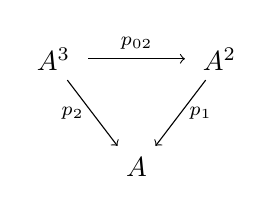
\begin{tikzpicture}[x=1.25em,y=1.4em]
  \node (A3) at (0,1.5) {$A^{3}$};
  \node (A2) at (4.8,1.5) {$A^{2}$};
  \node (A) at (2.4,-1.3) {$A$};
  \draw[->] (1.0,1.5) -- node[above]{$\scriptstyle p_{02}$} (3.8,1.5);
  \draw[->] (0.4,0.95) -- (1.85,-0.75);
  \node at (0.55,0.1) {$\scriptstyle p_{2}$};
  \draw[->] (4.4,0.95) -- (2.95,-0.75);
  \node at (4.25,0.1) {$\scriptstyle p_{1}$};
\end{tikzpicture}
\end{center}
在 $a\colon\qcOne\to A$ 之上的诸\trFiber{}上诱导的映射。余定义域投影
$p_{1}\colon\mathrm{Hom}_{A}(A,a)^{2}\to\mathrm{Hom}_{A}(A,a)$ 类似地等价于%
\trFibered{}投影映射 $p_{12}\colon A^{3}\to A^{2}$ 沿 $a\colon\qcOne\to A$ 的拉回。

把这些拼在一起，逗号∞-范畴
$\mathrm{Hom}_{\mathrm{Hom}_{A}(A,a)}(f_{*},\mathrm{Hom}_{A}(A,a))$ 便等价于下图
之极限：
\begin{center}
\begin{tikzpicture}[x=1.6em,y=1.6em]
  \node (dot) at (0,0) {$\bullet$};
  \node (Asq) at (3.0,0) {$A^{\ShapeSquare}$};
  \node (A3) at (6.0,0) {$A^{3}$};
  \node (A2t) at (9.4,0) {$A^{2}$};
  \node (A3m) at (3.0,-2.3) {$A^{3}$};
  \node (A2m) at (6.0,-2.3) {$A^{2}$};
  \node (One) at (0,-4.6) {$\qcOne$};
  \node (A2b) at (3.0,-4.6) {$A^{2}$};
  \draw[->] (0.5,0) -- (2.1,0);
  \draw[->] (3.9,0) -- (5.1,0);
  \draw[->] (6.9,0) -- node[above]{$\scriptstyle p_{12}$} (8.5,0);
  \draw[->] (0,-0.55) -- (0,-4.05);
  \draw[->] (3.0,-0.55) -- (3.0,-1.75);
  \draw[->] (6.0,-0.55) -- node[right]{$\scriptstyle p_{02}$} (6.0,-1.75);
  \node at (1.55,-0.75) {$\scriptstyle\lrcorner$};
  \node at (4.55,-0.75) {$\scriptstyle\lrcorner$};
  \draw[->] (3.9,-2.3) -- node[above]{$\scriptstyle p_{02}$} (5.1,-2.3);
  \draw[->] (3.0,-2.85) -- node[left]{$\scriptstyle p_{12}$} (3.0,-4.05);
  \draw[->] (0.55,-4.6) -- node[below]{$\scriptstyle f$} (2.1,-4.6);
\end{tikzpicture}
\end{center}
余定义域投影
$p_{1}\colon\mathrm{Hom}_{\mathrm{Hom}_{A}(A,a)}(f_{*},\mathrm{Hom}_{A}(A,a))\to\mathrm{Hom}_{A}(A,a)$
是上图顶部水平复合沿包含 $\mathrm{Hom}_{A}(A,a)\to A^{2}$ 的拉回。于是，逗号
∞-范畴 $\mathrm{Hom}_{\mathrm{Hom}_{A}(A,a)}(f_{*},g)$ 等价于左下方的极限，后者
重排为定义\trFiber{} $A^{\ShapeSquare}_{g\vee f}$ 的右下方拉回，这就证明了所宣称
的等价：
\begin{center}
\begin{tikzpicture}[x=1.6em,y=1.6em]
  \node (dot1) at (0,2.3) {$\bullet$};
  \node (dot2) at (3.0,2.3) {$\bullet$};
  \node (Onet) at (9.4,2.3) {$\qcOne$};
  \node (dotb) at (0,0) {$\bullet$};
  \node (Asq) at (3.0,0) {$A^{\ShapeSquare}$};
  \node (A3) at (6.0,0) {$A^{3}$};
  \node (A2t) at (9.4,0) {$A^{2}$};
  \node (A3m) at (3.0,-2.3) {$A^{3}$};
  \node (A2m) at (6.0,-2.3) {$A^{2}$};
  \node (One) at (0,-4.6) {$\qcOne$};
  \node (A2b) at (3.0,-4.6) {$A^{2}$};
  \draw[->] (0.5,2.3) -- (2.1,2.3);
  \draw[->] (3.9,2.3) -- (8.5,2.3);
  \draw[->] (9.4,1.75) -- node[right]{$\scriptstyle g$} (9.4,0.55);
  \draw[->] (0.5,0) -- (2.1,0);
  \draw[->] (3.9,0) -- (5.1,0);
  \draw[->] (6.9,0) -- node[above]{$\scriptstyle p_{12}$} (8.5,0);
  \draw[->] (0,-0.55) -- (0,-4.05);
  \draw[->] (3.0,-0.55) -- (3.0,-1.75);
  \draw[->] (6.0,-0.55) -- node[right]{$\scriptstyle p_{02}$} (6.0,-1.75);
  \node at (1.55,-0.75) {$\scriptstyle\lrcorner$};
  \node at (4.55,-0.75) {$\scriptstyle\lrcorner$};
  \draw[->] (3.9,-2.3) -- node[above]{$\scriptstyle p_{02}$} (5.1,-2.3);
  \draw[->] (3.0,-2.85) -- node[left]{$\scriptstyle p_{12}$} (3.0,-4.05);
  \draw[->] (0.55,-4.6) -- node[below]{$\scriptstyle f$} (2.1,-4.6);
\end{tikzpicture}
\qquad
\begin{tikzpicture}[x=1.5em,y=1.5em]
  \node (tl) at (0,1.5) {$A^{\ShapeSquare}_{g\vee f}$};
  \node (tr) at (5.4,1.5) {$A^{\ShapeSquare}$};
  \node (bl) at (0,-1.5) {$\qcOne$};
  \node (br) at (5.4,-1.5) {$A^{\ShapeCospan}$};
  \draw[->] (1.75,1.5) -- (3.9,1.5);
  \draw[->] (0,0.9) -- (0,-0.9);
  \node at (1.5,0.1) {$\scriptstyle\lrcorner$};
  \draw[->] (5.4,0.9) -- node[right]{$\scriptstyle\mathrm{res}$} (5.4,-0.9);
  \draw[->] (1.0,-1.5) -- node[below]{$\scriptstyle g\vee f$} (4.5,-1.5);
\end{tikzpicture}
\end{center}
\end{proof}

单纯集 $2\times2$ 有一个非恒同的自同构，它诱导 $A^{\ShapeSquare}$ 的一个
「转置」自同构。由对称性，$A$ 中的一个交换方块是拉回方块，当且仅当其转置方块是
拉回方块。这给出\cref{lem:pullbacks-as-absolute-liftings}的一个对偶形式，其中
$f$ 与 $g$ 的角色以及 $u$ 与 $v$ 的角色互换。作为推论，我们可以轻松证明：拉回
方块既可「竖直」复合又可「水平」复合，并且可以从「右边」与「底部」消去。

\begin{proposition}[拉回方块的复合与消去]\label{prop:pullback-square-cancelation}
给定 $A$ 中一个可复合的交换方块对及其复合矩形——后者经由等价
$A^{3\times 2}\simeq A^{\ShapeSquare}\times_{A^{2}}A^{\ShapeSquare}$ 定义——
\begin{center}
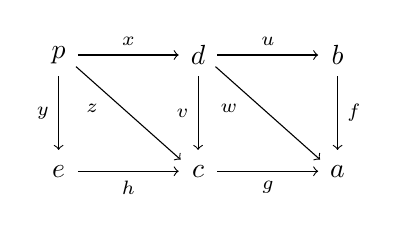
\begin{tikzpicture}[x=1.4em,y=1.4em]
  \node (p) at (0,1.8) {$p$};
  \node (d) at (3.6,1.8) {$d$};
  \node (b) at (7.2,1.8) {$b$};
  \node (e) at (0,-1.2) {$e$};
  \node (c) at (3.6,-1.2) {$c$};
  \node (a) at (7.2,-1.2) {$a$};
  \draw[->] (0.5,1.8) -- node[above]{$\scriptstyle x$} (3.1,1.8);
  \draw[->] (4.1,1.8) -- node[above]{$\scriptstyle u$} (6.7,1.8);
  \draw[->] (0,1.25) -- node[left]{$\scriptstyle y$} (0,-0.65);
  \draw[->] (3.6,1.25) -- node[left]{$\scriptstyle v$} (3.6,-0.65);
  \draw[->] (7.2,1.25) -- node[right]{$\scriptstyle f$} (7.2,-0.65);
  \draw[->] (0.5,-1.2) -- node[below]{$\scriptstyle h$} (3.1,-1.2);
  \draw[->] (4.1,-1.2) -- node[below]{$\scriptstyle g$} (6.7,-1.2);
  \draw[->] (0.45,1.5) -- node[pos=0.3,below left]{$\scriptstyle z$} (3.15,-0.9);
  \draw[->] (4.05,1.5) -- node[pos=0.3,below left]{$\scriptstyle w$} (6.75,-0.9);
\end{tikzpicture}
\end{center}
若右边的方块是拉回方块，则左边的方块是拉回方块，当且仅当复合矩形是拉回方块。
\end{proposition}

\begin{proof}
依\cref{lem:pullbacks-as-absolute-liftings}，我们给定一个绝对右提升图表
\begin{center}
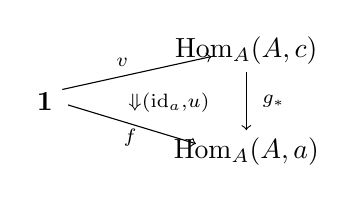
\begin{tikzpicture}[x=1.4em,y=1.4em]
  \node (Hc) at (5.2,1.7) {$\mathrm{Hom}_{A}(A,c)$};
  \node (One) at (0,0.4) {$\qcOne$};
  \node (Ha) at (5.2,-0.9) {$\mathrm{Hom}_{A}(A,a)$};
  \draw[->] (0.45,0.7) -- (4.3,1.55);
  \node at (2.0,1.4) {$\scriptstyle v$};
  \node at (3.2,0.35) {$\scriptstyle\Downarrow(\mathrm{id}_{a},u)$};
  \draw[->] (5.2,1.15) -- (5.2,-0.35);
  \node at (5.9,0.4) {$\scriptstyle g_{*}$};
  \draw[->] (0.6,0.3) -- (3.9,-0.7);
  \node at (2.2,-0.55) {$\scriptstyle f$};
\end{tikzpicture}
\end{center}
依引理 2.4.1，复合图
\begin{center}
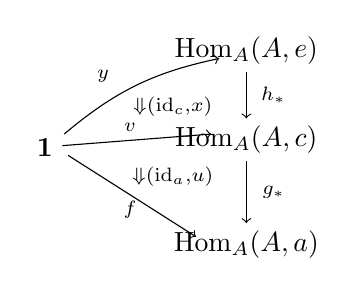
\begin{tikzpicture}[x=1.4em,y=1.4em]
  \node (He) at (5.2,3.4) {$\mathrm{Hom}_{A}(A,e)$};
  \node (Hc) at (5.2,1.1) {$\mathrm{Hom}_{A}(A,c)$};
  \node (Ha) at (5.2,-1.6) {$\mathrm{Hom}_{A}(A,a)$};
  \node (One) at (0,0.9) {$\qcOne$};
  \draw[->] (0.5,1.25) to[bend left=14] (4.5,3.2);
  \node at (1.5,2.75) {$\scriptstyle y$};
  \node at (3.3,1.95) {$\scriptstyle\Downarrow(\mathrm{id}_{c},x)$};
  \draw[->] (5.2,2.85) -- (5.2,1.65);
  \node at (5.9,2.25) {$\scriptstyle h_{*}$};
  \draw[->] (0.45,0.95) -- (4.3,1.25);
  \node at (2.2,1.42) {$\scriptstyle v$};
  \node at (3.3,0.15) {$\scriptstyle\Downarrow(\mathrm{id}_{a},u)$};
  \draw[->] (5.2,0.55) -- (5.2,-1.05);
  \node at (5.9,-0.25) {$\scriptstyle g_{*}$};
  \draw[->] (0.6,0.7) -- (3.9,-1.4);
  \node at (2.2,-0.7) {$\scriptstyle f$};
\end{tikzpicture}
\end{center}
是一个绝对右提升图表，当且仅当顶部的三角是绝对右提升图表。依%
\cref{lem:pullbacks-as-absolute-liftings}，这正是所要证明的。
\end{proof}

\begin{remark}\label{rem:x-indexed-pullback-squares}
\cref{prop:pullback-square-cancelation}的结果对 $X$-索引的交换方块族同样成立，
后者指\trDiagram{} $X\to A^{\ShapeSquare}$，或等价地，
$\mathrm{Fun}(X,A)^{\ShapeSquare}$ 的诸元素。证明相同，它利用%
\cref{lem:pullbacks-as-absolute-liftings}的一个推广：该推广断言，∞-宇宙
$\mathcal{K}$ 中取值于\trInfinityCategory{} $A$ 的、如下左图所示的 $X$-索引交换
方块是拉回方块，当且仅当如下右图所诱导的 2-胞腔 $(\mathrm{id}_{a},v)$ 是
$\mathcal{K}_{/X}$ 中的一个绝对右提升图表：
\begin{center}
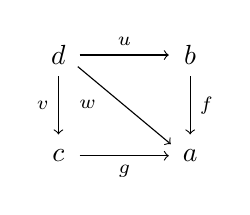
\begin{tikzpicture}[x=1.4em,y=1.4em]
  \node (d) at (0,1.7) {$d$};
  \node (b) at (3.4,1.7) {$b$};
  \node (c) at (0,-0.9) {$c$};
  \node (a) at (3.4,-0.9) {$a$};
  \draw[->] (0.55,1.7) -- node[above]{$\scriptstyle u$} (2.85,1.7);
  \draw[->] (0,1.15) -- node[left]{$\scriptstyle v$} (0,-0.35);
  \draw[->] (3.4,1.15) -- node[right]{$\scriptstyle f$} (3.4,-0.35);
  \draw[->] (0.55,-0.9) -- node[below]{$\scriptstyle g$} (2.85,-0.9);
  \draw[->] (0.5,1.4) -- node[pos=0.3,below left]{$\scriptstyle w$} (2.9,-0.6);
\end{tikzpicture}
\qquad
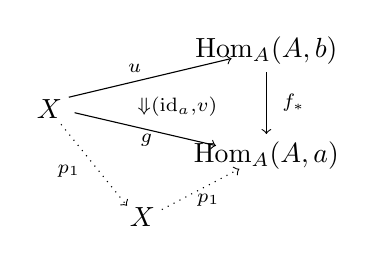
\begin{tikzpicture}[x=1.4em,y=1.4em]
  \node (Hb) at (5.6,1.9) {$\mathrm{Hom}_{A}(A,b)$};
  \node (Xm) at (0,0.4) {$X$};
  \node (Ha) at (5.6,-0.8) {$\mathrm{Hom}_{A}(A,a)$};
  \node (Xb) at (2.4,-2.4) {$X$};
  \draw[->] (0.5,0.7) -- (4.7,1.7);
  \node at (2.2,1.45) {$\scriptstyle u$};
  \node at (3.3,0.45) {$\scriptstyle\Downarrow(\mathrm{id}_{a},v)$};
  \draw[->] (5.6,1.35) -- (5.6,-0.25);
  \node at (6.3,0.55) {$\scriptstyle f_{*}$};
  \draw[->] (0.65,0.3) -- (4.3,-0.55);
  \node at (2.5,-0.4) {$\scriptstyle g$};
  \draw[->,dotted] (0.3,0.0) -- (2.0,-2.1);
  \node at (0.5,-1.2) {$\scriptstyle p_{1}$};
  \draw[->,dotted] (2.9,-2.2) -- (4.9,-1.15);
  \node at (4.1,-1.95) {$\scriptstyle p_{1}$};
\end{tikzpicture}
\end{center}
\end{remark}

对 $X$-索引拉回方块的这一刻画，可以通过在切片∞-宇宙 $\mathcal{K}_{/X}$ 中重新
实现\cref{lem:pullbacks-as-absolute-liftings}之证明所给的构造来证明——以逗号
∞-范畴与切片∞-宇宙 $\mathcal{K}_{/X}$ 中的单纯极限（如命题 1.2.22 所描述者）取代
$\mathcal{K}$ 中的类似构造。若非涉及的记号更为繁复，我们本会呈现这个一般证明而非
上面的特殊情形。

另一种做法是，这一扩展可以从我们在此证明的结果推导出来。$\mathcal{K}$ 中的一个%
\trDiagram{} $s\colon X\to A^{\ShapeSquare}$ 也定义了切片∞-宇宙 $\mathcal{K}_{/X}$
中以 $\pi\colon A\times X\to X$ 为取值的一个 $X$-索引交换方块，其形式为 $X$ 之上的
一个函子 $(s,\mathrm{id}_{X})\colon X\to A^{\ShapeSquare}\times X$。容易验证：
取值于 $\pi\colon A\times X\to X$ 且其在 $X$ 处的分量为恒同的\trDiagram{}在
$\mathcal{K}_{/X}$ 中有\trLimit{}，当且仅当该\trDiagram{}的 $A$ 分量在 $\mathcal{K}$
中有\trLimit{}。由于 $\mathrm{id}_{X}$ 是 $\mathcal{K}_{/X}$ 的\trTerminal{}对象，
这个对象就是 $\mathcal{K}_{/X}$ 中的∞-范畴 $1$，故%
\cref{lem:pullbacks-as-absolute-liftings}在切片∞-宇宙 $\mathcal{K}_{/X}$ 中适用，
从而证明了 $\mathcal{K}$ 中 $X$-索引交换方块族的一般情形。

正如例 2.3.10 所讨论的，\trTerminal{}\trElement{}与\trInitial{}\trElement{}分别
是\trLimit{}与\trColimit{}的特殊情形，其中\trDiagram{}形状为空。
对任何\trInfinityCategory{} $A$，$A$ 中诸\trEmptyDiagram{}的∞-范畴
$A^{\emptyset}\cong\qcOne$ 是\trTerminal{}的。于是，$A$ 中存在唯一的
$\emptyset$-索引\trDiagram{}。由定义 4.2.1 中逗号∞-范畴的构造立即可知：唯一空%
\trDiagram{}之上与之下二者的\trInfinityCategoryOfCones{}都同构于 $A$。
在空\trDiagram{}之上的\trCone{}的情形，把\trCone{}送到其顶点的定义域求值函子在
$A$ 上是恒同；而在空\trDiagram{}之下的\trCone{}的情形，把\trCone{}送到其\trNadir{}的
余定义域求值函子在 $A$ 上是恒同。
下面这个关于\trTerminal{}\trElement{}的刻画可以当作%
\cref{prop:colimits-represent-cones}的特殊情形推导出来，不过我们发现从命题 4.1.1
出发论证更为容易。

\begin{proposition}\label{prop:terminal-initial-trivial-fibration}
\trInfinityCategory{} $A$ 的一个\trElement{} $a\colon\qcOne\to A$
(i) 定义 $A$ 的一个\trTerminal{}\trElement{}，当且仅当定义域投影函子
$p_{0}\colon\mathrm{Hom}_{A}(A,a)\twoheadrightarrow A$ 是一个平凡纤维化；而
(ii) 定义 $A$ 的一个\trInitial{}\trElement{}，当且仅当余定义域投影函子
$p_{1}\colon\mathrm{Hom}_{A}(a,A)\twoheadrightarrow A$ 是一个平凡纤维化。
\end{proposition}

\begin{proof}
回顾定义 2.2.1：一个\trElement{}是\trTerminal{}的，当且仅当它是唯一函子
\begin{center}
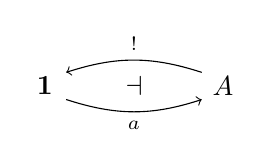
\begin{tikzpicture}[x=1.4em,y=1.4em]
  \node (One) at (0,0) {$\qcOne$};
  \node (A) at (4.6,0) {$A$};
  \draw[->] (4.05,0.35) to[bend right=18] node[above]{$\scriptstyle !$} (0.55,0.35);
  \node at (2.3,0) {$\dashv$};
  \draw[->] (0.55,-0.35) to[bend right=18] node[below]{$\scriptstyle a$} (4.05,-0.35);
\end{tikzpicture}
\end{center}
的\trRightAdjoint{}。依命题 4.1.1，$!\dashv a$ 当且仅当存在等价
$\mathrm{Hom}_{\qcOne}(!,\qcOne)\simeq_{A}\mathrm{Hom}_{A}(A,a)$。依逗号∞-范畴的
定义性拉回 (3.4.2)，$!\colon A\to\qcOne$ 的左表示就是 $A$ 本身，其定义域投影函子
为恒同。
于是，等价 $\mathrm{Hom}_{A}(A,a)\twoheadrightarrow A$ 在 $A$ 之上的分量必为定义域投影
函子 $p_{0}\colon\mathrm{Hom}_{A}(A,a)\twoheadrightarrow A$，故我们得出：$a$ 是一个%
\trTerminal{}\trElement{}，当且仅当这一等价纤维化是一个平凡纤维化。
\end{proof}

\begin{digression}[\trQuasiCategory{}的\trTerminal{}\trElement]\label{dig:terminal-elements-quasi-category}
在\trQuasiCategory{}的\trInfinityCosmos{}中，等价纤维化
$p_{0}\colon\mathrm{Hom}_{A}(A,a)\allowbreak\twoheadrightarrow\allowbreak A$ 之定义域在 $A$ 上等价于切片拟范畴
$A_{/a}$——后者由命题 4.2.5 定义（见推论 D.6.6）。
经由这一等价，\cref{prop:terminal-initial-trivial-fibration}证明了：$a$ 是一个%
\trTerminal{}\trElement{}，当且仅当投影 $A_{/a}\to A$ 是定义 1.1.25 意义下的平凡
纤维化，而这转置后即为 Joyal 关于拟范畴之终元素的原始定义。扩充的讨论见命题
F.1.1。
\end{digression}

\subsection*{练习}

\begin{exercise}[函子\trInfinityCategory{}中的逐点\trLimit]\label{ex:pointwise-limits}
设 $A$ 容许一族形状为 $J$ 的\trDiagram{} $d\colon D\to A^{J}$ 的\trLimit{}
$\ell\colon D\to A$。证明：\trDiagram{}∞-范畴 $A^{K}$ 容许相应的 $J$ 形状%
\trDiagram{}族 $d^{K}\colon D^{K}\to(A^{J})^{K}\cong(A^{K})^{J}$ 的\trLimit{}，后者
由函子 $\ell^{K}\colon D^{K}\to A^{K}$「在 $K$ 中逐点」定义。%
\footnote{若 $K$ 是\trCartesianClosed{}\trInfinityCosmos{} $\mathcal{K}$ 中的一个%
\trInfinityCategory{}，这可以在\trHomotopyTwoCategory{}中论证而直接证明；但另一个
证明同时适用于此情形与 $K$ 为\trSimplicialSet{}的情形：利用宇宙论函子
$(-)^{K}\colon\mathcal{K}\to\mathcal{K}$ 保持\cref{prop:colimits-represent-cones}
之等价这一事实。}
\end{exercise}

\begin{exercise}\label{ex:j-indexed-versions}
陈述并证明\cref{prop:absolute-right-lifting-res}与\cref{cor:res-fibered-adjoints}
的版本，使之适用于\trCartesianClosed{}\trInfinityCosmos{}中由一个%
\trInfinityCategory{} $J$ 索引的\trDiagram{}族 $d\colon D\to A^{J}$。
\end{exercise}

\begin{exercise}\label{ex:tensor-associativity}
设 $a$ 为\trInfinityCategory{} $A$ 的一个\trElement{}，并设 $K$ 与 $L$ 为单纯集。
证明：若 $A$ 具有\trTensor{}与\trCotensor{}，则这些运算是结合的，其意义是：元素
\begin{equation*}
K\otimes(L\otimes a)\cong(K\times L)\otimes a\cong L\otimes(K\otimes a)
\qquad\text{与}\qquad
(a^{L})^{K}\cong a^{K\times L}\cong(a^{K})^{L}
\end{equation*}
是同构的。
\end{exercise}

\begin{exercise}\label{ex:mapping-space-contractible}
证明：若 $A$ 有一个\trTerminal{}\trElement{} $t$，则对任何\trElement{} $a$，
\trMappingSpace{} $\mathrm{Hom}_{A}(a,t)$ 是\textbf{可缩的}（contractible），即
等价于终∞-范畴 $\qcOne$。%
\footnote{逆命题在 $(\infty,1)$-范畴的\trInfinityCosmos{}中成立，论证见命题
F.1.1 的证明。}
\end{exercise}

\begin{exercise}\label{ex:family-pullback-criteria}
设 $A$ 容许\trPullback{}，并考虑交换方块族 $d\colon D\to A^{\ShapeSquare}$。证明
下列诸条等价：
(i) 交换三角
\begin{center}
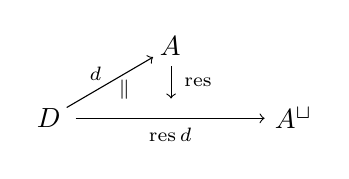
\begin{tikzpicture}[x=1.3em,y=1.3em]
  \node (Asq) at (3.4,2.0) {$A^{\ShapeSquare}$};
  \node (D) at (0,0) {$D$};
  \node (Acup) at (6.8,0) {$A^{\ShapeCospan}$};
  \draw[->] (0.5,0.3) -- (2.9,1.7);
  \node at (1.3,1.25) {$\scriptstyle d$};
  \node at (2.1,0.8) {$\scriptstyle\parallel$};
  \draw[->] (3.4,1.45) -- (3.4,0.55);
  \node at (4.15,1.0) {$\scriptstyle\mathrm{res}$};
  \draw[->] (0.75,0) -- node[below]{$\scriptstyle\mathrm{res}\,d$} (6.0,0);
\end{tikzpicture}
\end{center}
是一个绝对右提升图表。
(ii) \trAdjunction{} $\mathrm{res}\dashv\mathrm{ran}$ 之\trUnit{}的分量
\begin{center}
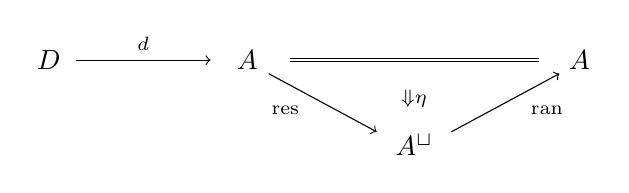
\begin{tikzpicture}[x=1.5em,y=1.4em]
  \node (D) at (0,0) {$D$};
  \node (AsqL) at (4.8,0) {$A^{\ShapeSquare}$};
  \node (AsqR) at (12.8,0) {$A^{\ShapeSquare}$};
  \node (Acup) at (8.8,-2.2) {$A^{\ShapeCospan}$};
  \draw[->] (0.65,0) -- node[above]{$\scriptstyle d$} (3.9,0);
  \draw[double] (5.8,0) -- (11.8,0);
  \draw[->] (5.3,-0.35) -- (7.9,-1.85);
  \node at (5.7,-1.3) {$\scriptstyle\mathrm{res}$};
  \node at (8.8,-1.0) {$\scriptstyle\Downarrow\eta$};
  \draw[->] (9.7,-1.85) -- (12.3,-0.35);
  \node at (12.0,-1.3) {$\scriptstyle\mathrm{ran}$};
\end{tikzpicture}
\end{center}
可逆。
\end{exercise}

\begin{exercise}\label{ex:transposed-pullback}
证明：$A$ 中的一个方块是拉回方块，当且仅当其「转置」方块是拉回方块——后者由与
对合 $A^{\ShapeSquare}\cong A^{\ShapeSquare}$ 复合而定义，该对合由 $2\times 2$ 的
交换「非对角」元素的自同构诱导。
\end{exercise}

\begin{exercise}\label{ex:binary-products-pullbacks}
证明：任何具有\trPullback{}与一个\trTerminal{}\trElement{}的\trInfinityCategory{}%
都容许二元积。
\end{exercise}
